\documentclass[a4paper,kulak]{kulakarticle}

\usepackage[utf8]{inputenc}
\usepackage[dutch]{babel}
\usepackage{pdfpages}
\usepackage{subfig}
\usepackage{float}

\usepackage{cite}

% style
%\usepackage[left=2.5cm,top=2cm,right=2.5cm,bottom=2cm,a4paper]{geometry}
\usepackage{color}

\date{\today}
\address{
	Bachelor in de fysica\\
	Bachelor in de informatica\\
	Bachelor in de wiskunde\\
	Ingenieurswetenschappen}
\title{BDA App}
\author{Marthe B\"{o}ting\\
	Robin Bruneel\\
	Toon Ingelaere}

\begin{document}
	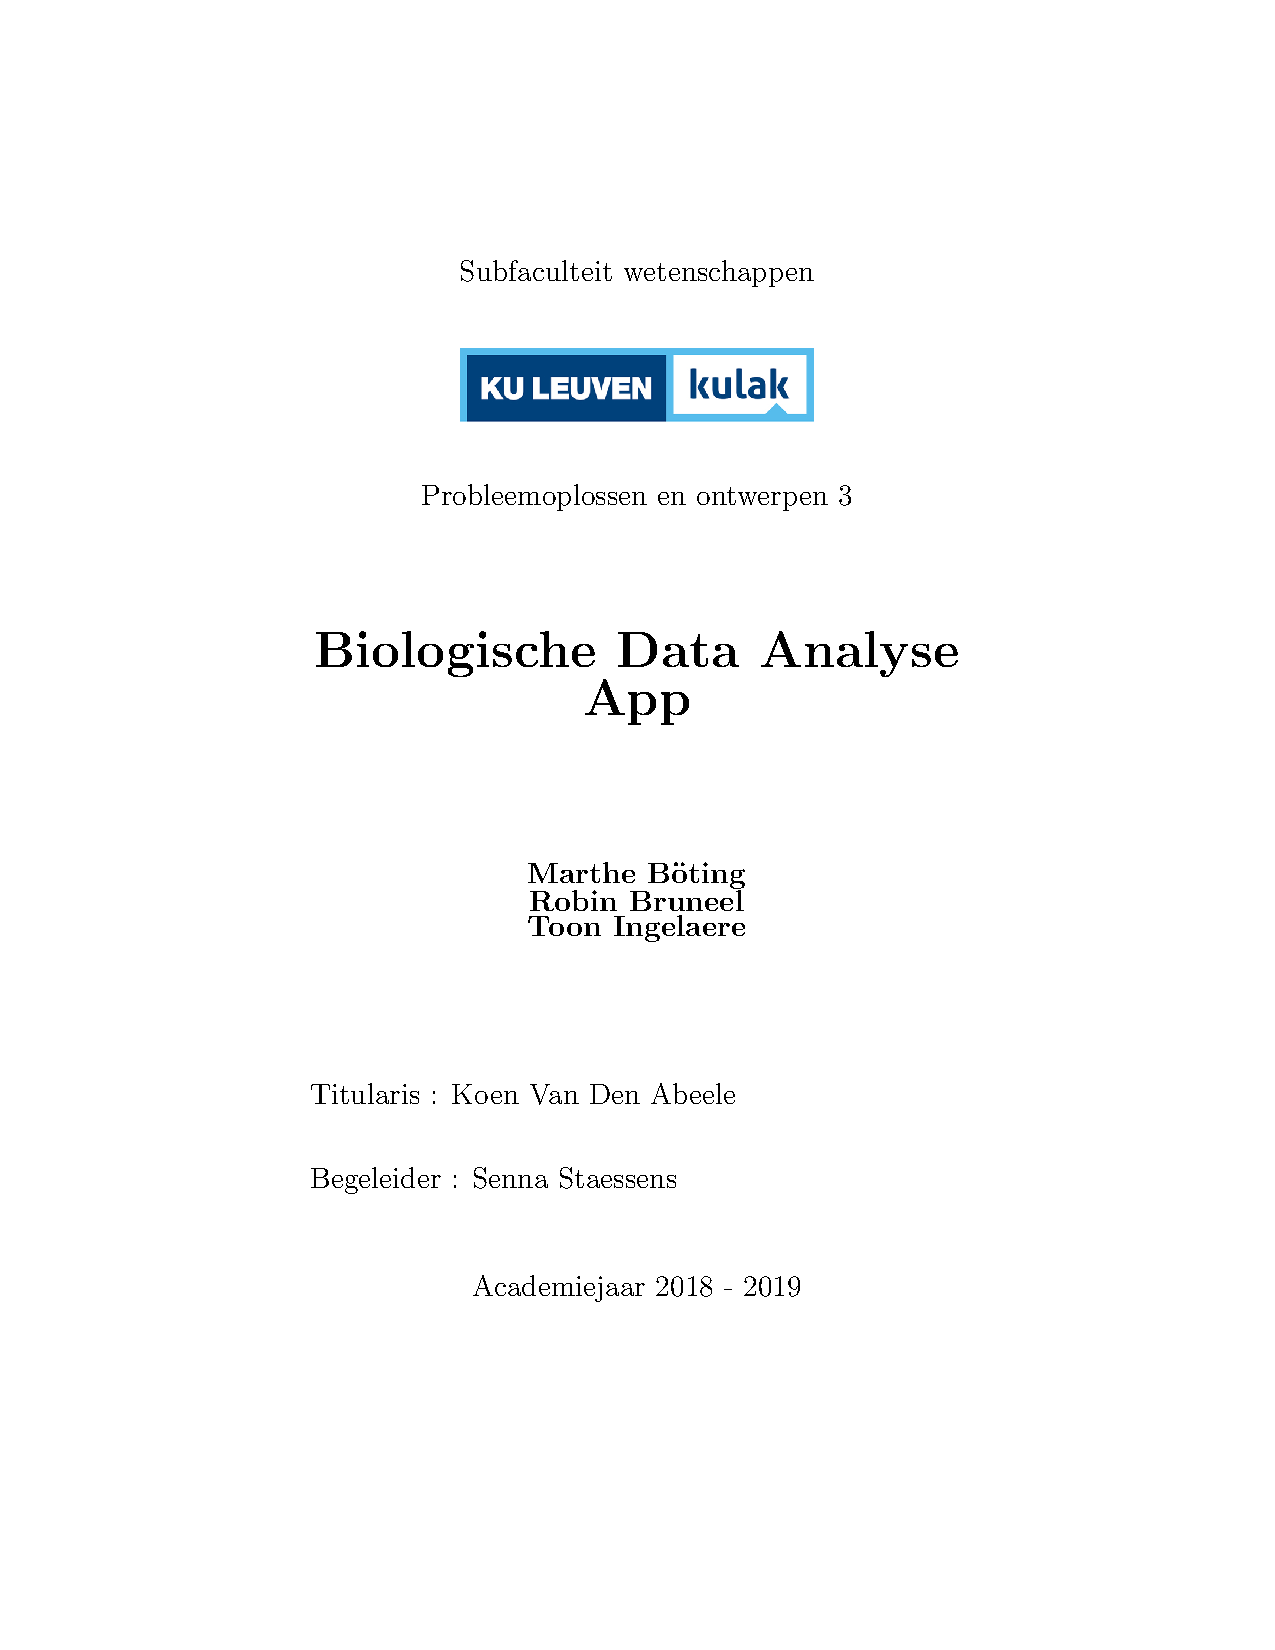
\includepdf{voorblad}
	
	\maketitle

\section*{Inleiding}

<<<<<<< HEAD
Inleidende tekst.

\tableofcontents

\section{ISectie-titel}
=======
Beroertes zijn in onze westerse samenleving de derde grootste doodsoorzaak na hartinfarcten en kanker. Zoals we zien op Figuur \ref{figuur doodsoorzaken} kapen ze op wereldvlak zelfs de tweede plaats weg\cite{worldhealthorganization}. In België komen er gemiddeld 25 000 beroertes per jaar voor. In 15\% van deze gevallen overlijdt de patiënt. De overige 85\% heeft na een beroerte vaak last van blijvende functiebeperkingen zoals cognitieve-, emotionele of gedragsproblemen. Een ischemische beroerte ontstaat doordat een bloedklonter emboliseert en in één van de hersenbloedvaten vast komt te zitten. Deze bloedklonter moet verwijderd worden of de patiënt loopt een hersenschade op.
Momenteel focust de huidige therapie zich op snel en efficiënt verwijderen van de bloedklonter. In eerste instantie kan men via een geneesmiddel, weefsel plasminogeen activator, proberen om de klonter op te lossen. Dit geneesmiddel moet gegeven worden binnen de eerste 4,5 uur na het optreden van de symptomen. Wanneer dit geneesmiddel wordt toegediend na dit tijdstip kan dit leiden tot bloedingen of toxiciteit in de hersenen. Van alle patiënten die het geneesmiddel toegediend krijgen, lost de klonter slechts in 1/3 van de patiënten op.
Op het moment dat de klonter niet oplost , maakt men gebruik van trombectomie om de klonter er manueel uit te halen.
Om huidige therapeutische opties te verbeteren en om het aantal slachtoffers aan beroertes te doen slinken, gebruikt men deze bloedklonters om verder onderzoek op uit te voeren. Hiervoor gaan ze de samenstelling van de bloedklonter proberen te analyseren. Dit gebeurt op basis van afbeeldingen die gemaakt zijn van de bloedklonter waarbij welbepaalde componenten gekleurd zijn (bijvoorbeeld: rode bloedcellen, witte bloedcellen en bloedplaatjes) en vervolgens geanalyseerd worden via kleur-gebaseerde segmentatie analyse.
Deze analyses zijn echter erg tijdrovend. Er is ons dan ook gevraagd om een gebruiksvriendelijke app te ontwikkelen die de analyse van de afbeeldingen kan automatiseren.
In dit verslag gaan we eerst in op wat de klant specifiek van ons verwacht en aan welke specificaties ons ontwerp moet voldoen. Hierna bespreken we ons design en lichten we het toe. Verder bespreken we ook enkele van onze voorlopige resultaten. Ten slotte wordt er nog een blik geworpen naar de vakken uit eerste drie semesters die ons hierbij geholpen hebben.

	\begin{figure}[H]
		\centering
		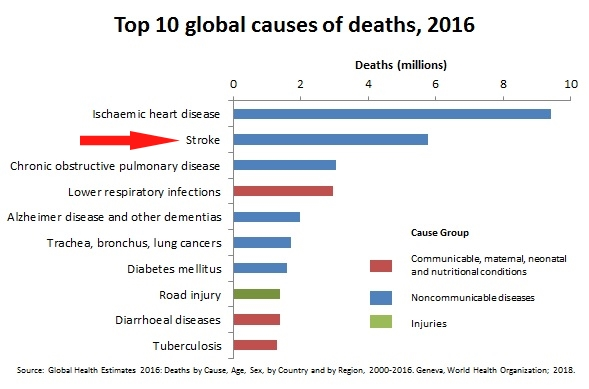
\includegraphics[width = 0.7\textwidth]{top10doodsoorzaken.png}
	
		\caption{Statistieken van de \textit{World Health Organization} van 2016 waarin te zien is dat wereldwijd beroertes (\textit{strokes}) de tweede meest frequente doodsoorzaak is.}
		\label{figuur doodsoorzaken}
	\end{figure}

\pagebreak
\newpage

\tableofcontents

\newpage
>>>>>>> master

\section{Klantenvereisten}
De klant verwacht een gebruiksvriendelijke app die de afbeeldingen automatisch verwerkt. Dit houdt in dat een afbeelding ingeladen kan worden, de foto bijgesneden en de achtergrond verwijderd wordt. Daarnaast is het de bedoeling om de samenstelling van de bloedklonter te analyseren aan de hand van de aangebrachte indicator.

\section{Ontwerpspecificatie}
De klant wil dat een afbeelding van een bloedklonter automatisch bewerkt en daarna geanalyseerd wordt.\\
Het bewerken van de afbeelding houdt twee dingen in. Eerst en vooral moet de afbeelding zodanig bijgesneden worden dat de volledige bloedklonter erop staat. Hierbij mogen we de randen echter niet te breed nemen, aangezien er dan nuttige geheugenruimte\footnote{We werken namelijk met foto's van de orde van 200MB, het sparen van pixels op ons resultaat is uiterst voordelig} verspild wordt. 
Naast het bijsnijden, moet ook de achtergrond verwijderd worden. Dit betekent dat alle pixels die niet tot de bloedklonter behoren wit gekleurd worden. Indien dit niet goed gebeurt, kunnen de resultaten van de kleurenanalyse namelijk vertekend zijn.\\
In de kleurenanalyse moet het percentage van met indicator gekleurde pixels geteld worden. Voor dit project moeten we slechts twee soorten kleuringen analyseren. Een voorbeeld van deze is te zien in Figuur \ref{figuur indicators}. In beide gevallen moet de app op een accurate manier onderscheid kunnen maken tussen de eiwitten die gedetecteerd moeten worden en de rest van de bloedklonter. \\
Dit alles moet samengegoten worden in een visuele en gebruiksvriendelijke app. Dit wil zeggen dat de app makkelijk te installeren en te gebruiken is. De gebruiker moet ook een overzicht van de verschillende afbeeldingen van de bloedklonter kunnen terugroepen. Dit overzicht bestaat uit de originele afbeelding, de afbeelding zonder achtergrond en de afbeelding waarbij de indicatorpixels zijn aangeduid. Zo kunnen mogelijke fouten snel gedetecteerd worden. Daarnaast moet deze app nog wat extra functionaliteiten uitvoeren zoals het opslaan van deze afbeeldingen, het manueel bijwerken van het bekomen resultaat, het wegschrijven van alle data in een csv\footnote{Een csv (Comma Separated Values) bestand is een tekstbestand die als tabel ingelezen kan worden. Het kan eenvoudig in excel geopend worden voor verdere analyse.} bestand, etc.

\section{Onze oplossing}
Dit hoofdstuk hebben we opgedeeld in verschillende deelproblemen, namelijk het verwijderen van de achtergrond, het lokaliseren van de indicator en de gebruiksvriendelijke app. We zullen deze deelproblemen nader bespreken en onze bekomen bevindingen rapporteren. Om onze app te realiseren, maken we gebruik van de programmeertaal MATLAB.

	\subsection{Achtergrondverwijdering}
	Het eerste deelprobleem van ons project is het verwijderen van de achtergrond. Op de afbeeldingen is er heel wat vuiligheid te vinden. Voorbeelden hiervan zijn luchtbellen of kleine verkleuringen naast de bloedklonter zoals men ziet op de Figuur \ref{figuur achtergrondverwijdering}. Hieronder zullen we verschillende operaties beschrijven om de grootste klonters te lokaliseren en alles wat geen klonter is te verwijderen. Dit leidt tot een ruisvrije afbeelding.
	
	\begin{figure}[H]
		\centering
		\includegraphics[width = 0.7\textwidth]{Ruis_afbeelding.png}	
		\caption{In de rechterbovenhoek zien we luchtbellen en in de onderste cirkel zien we een verkleuring die geen deel uitmaakt van een bloedklonter.}
		\label{figuur achtergrondverwijdering}
	\end{figure}

	\subsubsection{Bepalen van de beste threshold}
	Wanneer we de grijswaarden van de afbeelding berekenen, zien we een opmerkelijk verschil tussen de achtergrond (eerder wit) en de bloedklonter (eerder grijs),  zie Figuur \ref{figuur beste_threshold}. Wanneer we een histogram van deze grijswaarden opstellen, vinden we ook een lokaal minimum tussen het grijs en het wit. Dit zien we duidelijk op het histogram in Figuur \ref{figuur graf1}. Wanneer we dit minimum berekenen, vinden we de theoretisch optimale threshold, de grijswaarde om een bloedklonterpixel van een achtergrondpixel te onderscheiden. Wanneer we die threshold toepassen en een binaire representatie zoals in Figuur \ref{figuur foto_bin} vormen, zien we namelijk dat dit inderdaad een goede threshold is.
	
	\begin{figure}[H]
		\centering
		\subfloat[]{{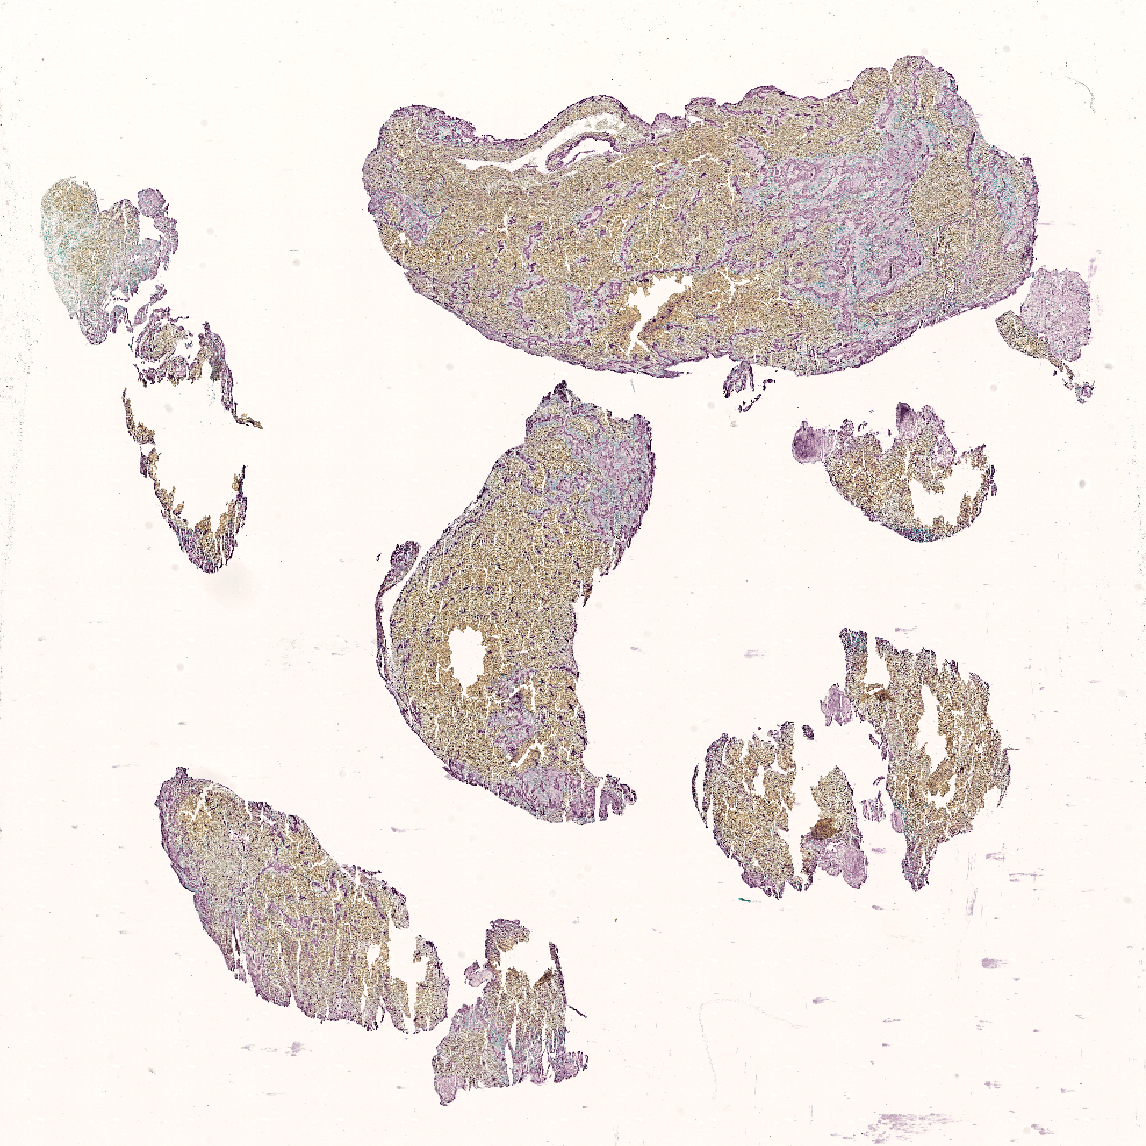
\includegraphics[width=6cm]{origineel_vb}}}
		\qquad
		\subfloat[]{{\includegraphics[width=6cm]{grijswaarden_vb}}}
		
		\caption{Illustratie van de originele foto (a) en deze omgezet in grijswaarden (b).}
		\label{figuur beste_threshold}
	\end{figure}
	
	\begin{figure}[H]
		\centering
		\includegraphics[width=0.85\textwidth]{GetBestthreshold_vb_aangeduid.png}
		
		\caption{Histogram van het aantal pixels gegroepeerd per grijswaarde. We zien duidelijk een lokaal minimum rond de waarde 230. Opmerking: we maken hier gebruik van een logaritmische y-as.}
		\label{figuur graf1}
	\end{figure}
	
	\begin{figure}[H]
		\centering
		\includegraphics[width=0.7\textwidth]{grijswaarden_bin_vb}
		\caption{Op deze binaire representatie zijn de bloedklonters duidelijk te zien.}
		\label{figuur foto_bin}
	\end{figure}


\subsection{De gebruiksvriendelijke applicatie}
De app werkt op basis van de klant die een foto kan ingeven. Het resultaat is een bewerkte foto waarbij er een percentage van de hoeveelheid aanwezig kleur weergegeven wordt.\\
Op het moment dat de klant een afbeelding gekozen heeft, zal  in de eerste fase de achtergrond van de foto wit worden gemaakt en wordt de foto bijgesneden zodanig dat enkel de bloedklonter zichtbaar is. Als dit gebeurd is, zal er al een eerste resultaat getoond worden. Hierdoor heeft de klant een beeld waarop de verdere analyse zal gebeuren en kan die eventueel ingrijpen bij fouten. \\
Vervolgens zal de kleurenanalyse gebeuren. Ook hiervoor zal de foto getoond worden waarop de klant kan zien welke delen de indicator bevatten en zal het percentage gegeven worden. \\
Soms is de kleuring intenser dan anders dit is het gevolg van verschillende factoren (bijvoorbeeld: temperatuur, druk, vochtigheid,... ). Hierdoor kan het resultaat die wordt bekomen via de app eens afwijken van de werkelijke waarde. Daarom hebben wij sliders toegevoegd. Zoals eerder vermeld hebben wij experimenteel waarden bepaald waartussen gewerkt wordt. Door het toevoegen van deze sliders kan de klant zelf deze waarden aanpassen wanneer de kleuring afwijkt. Deze kunnen ook gebruikt worden op het moment dat de bewerkte foto .
Daarnaast is er de mogelijkheid aan om niet foto per foto in te geven maar een volledige map met foto's die dan elk afzonderlijk bewerkt en opgeslagen worden.

\section*{Besluit}

Afsluitende tekst

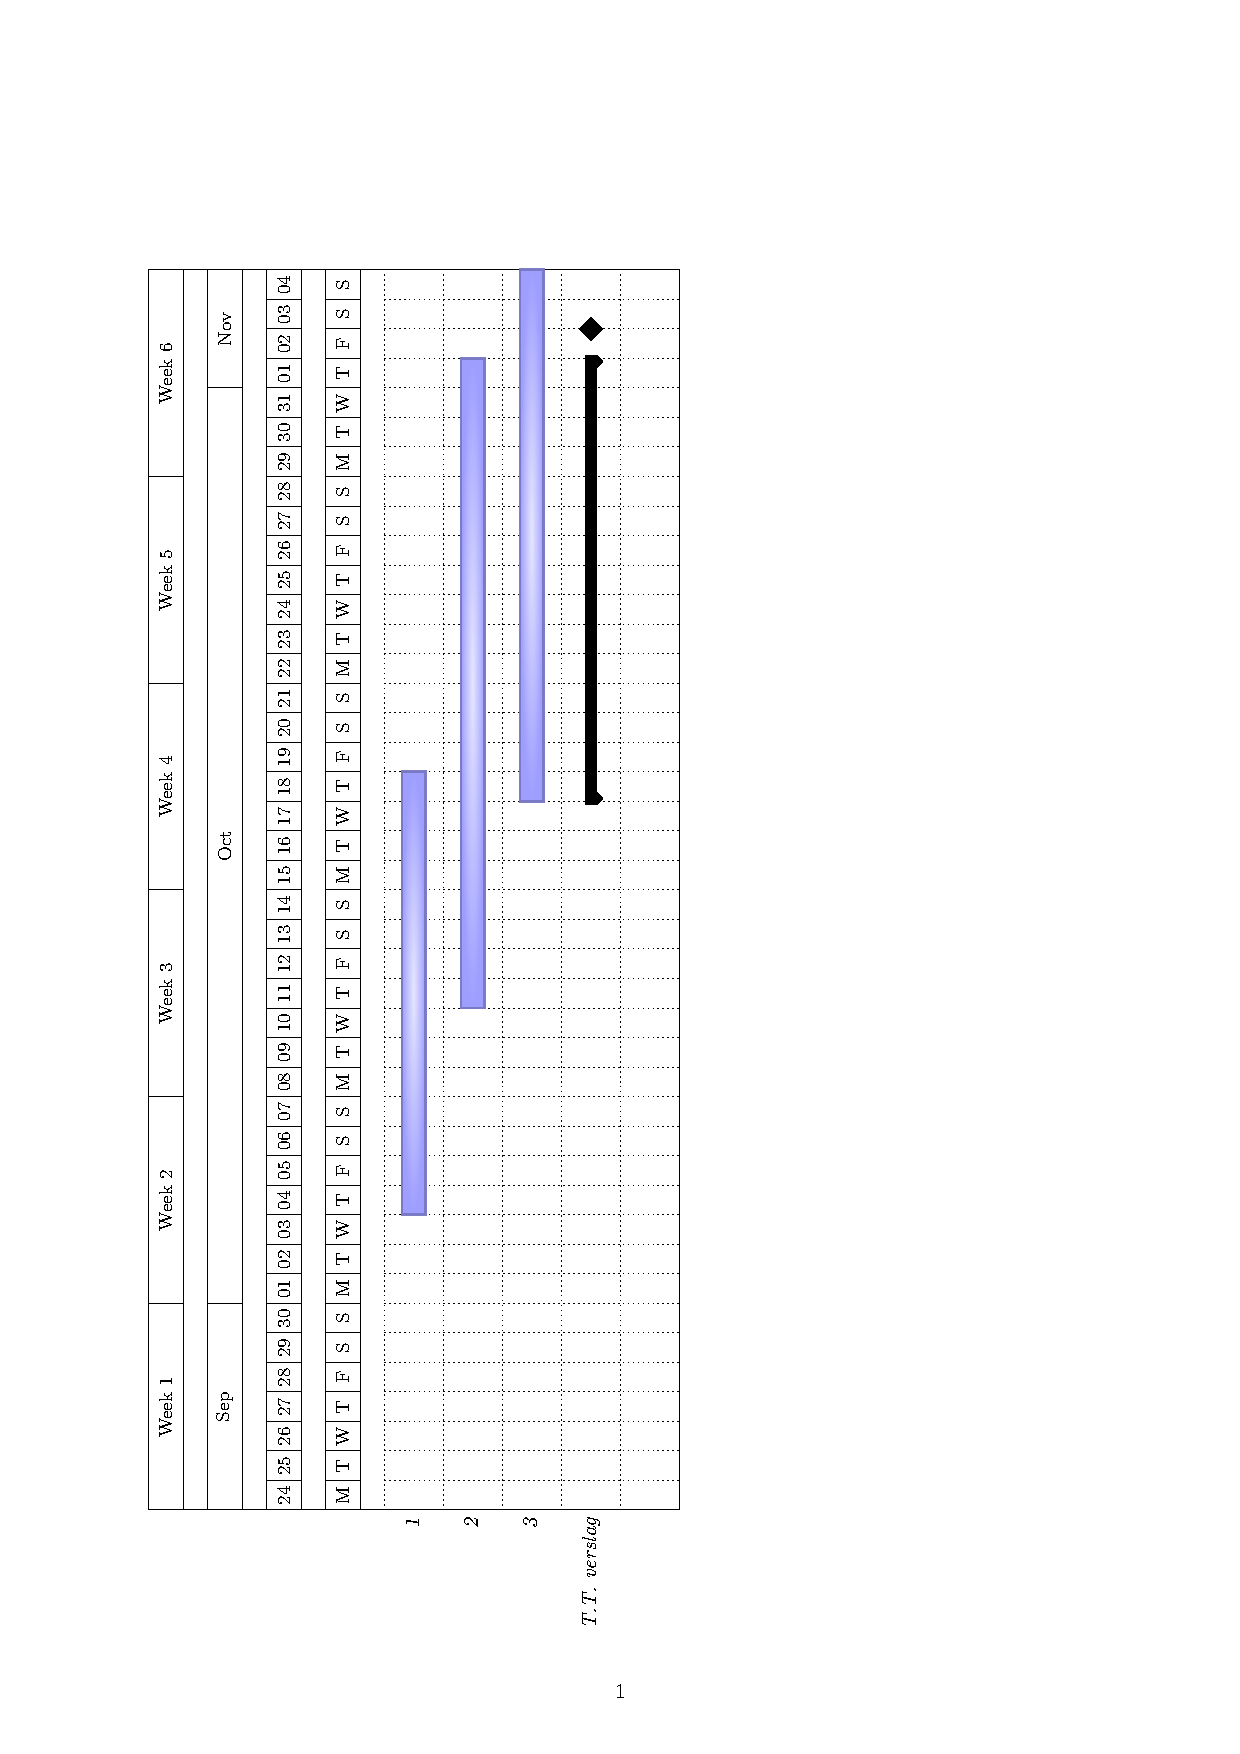
\includepdf[pages={1-3}]{ganttchart}

\end{document}
